% =============================================================================
% GPTI Project -- Deliverable P2B (English version of Projeto_GPTI_Entrega_P2B_PT-BR.tex)
% Formatting: ABNT (abnTeX2 class, article mode), A4, Latin Modern, 12 pt,
% margins 3/2/3/2 cm, 1.5 line spacing, 1.25 cm paragraph indent.
% Expected figure: out/Figura_1_Percurso_Dado_Pessoal_EN.pdf
% (compiled from figuras/Figura_1_Percurso_Dado_Pessoal_EN.tex)
% =============================================================================
\documentclass[12pt,a4paper,article,oneside,brazil,english]{abntex2}

\usepackage[T1]{fontenc}
\usepackage[utf8]{inputenc}
\usepackage{lmodern}           % Latin Modern (fonte padrão do LaTeX, com T1)
\usepackage{amsmath}
\usepackage{graphicx}
\usepackage{array}
\usepackage{tabularx}
\usepackage[expansion=false]{microtype}

% ABNT margins: top 3 cm, bottom 2 cm, left 3 cm, right 2 cm
\setlrmarginsandblock{3cm}{2cm}{*}
\setulmarginsandblock{3cm}{2cm}{*}
\checkandfixthelayout

\setlength{\parindent}{1.25cm}
\setlength{\parskip}{0pt}
\setlength{\emergencystretch}{2em}

% Tables: no vertical rules (IBGE standard adopted by ABNT)
\newcolumntype{Y}{>{\raggedright\arraybackslash}X}
\renewcommand{\arraystretch}{1.2}

% Source line below tables and figures (ABNT NBR 14724)
\newcommand{\fontetab}[1]{\par\vspace{3pt}{\small\noindent Source: #1\par}}

% Configuration DSQ(t_k)
\newcommand{\dsq}[1]{DSQ($t_{#1}$)}

\begin{document}

% ------------------------------- COVER ---------------------------------------
\thispagestyle{empty}
\noindent\begin{minipage}[t][0.92\textheight]{\textwidth}
\centering
\SingleSpacing
\textbf{UNIVERSITY OF BRASÍLIA -- UnB\\
GRADUATE PROGRAM IN APPLIED COMPUTING -- PPCA\\
COURSE: IT PROJECT MANAGEMENT (GPTI)\\
PROFESSOR: Dr. JOÃO MELLO DA SILVA}

\vspace{1cm}

\textbf{Digital Mobilizer 1 Group}: Gabriel Porto Oliveira, Marcus Vinícius Oliveira Reis, Suzy Alves Arcanjo and William de Almeida Silva.

\vspace{0.4cm}

\textbf{Recycling 1 Group:} Filipe Alves de Sousa, Emanuel Brandão de Galvão Correia, Ruben Isaac Dias da Silva and Carlos Eduardo da Silva Papa.

\vspace{0.4cm}

\textbf{Landfill Group:} Lucien Rocha, Edvan Silva, Helton Garcia and Lucas Ferreira.

\vspace{3cm}

\textbf{PRIVACY IN DIGITAL TWINS OF THE SOLID WASTE SYSTEM: FSPC CONSOLIDATION OF THREE SEGMENTS}

\vfill

BRASÍLIA -- DF\\
2026
\end{minipage}
\clearpage

% ------------------------------ ABSTRACTS ------------------------------------
\begin{resumo}[Abstract]
This paper consolidates three projects from the GPTI course that describe digital twins of successive segments of the Solid Waste System (SRS, from the Portuguese \textit{Sistema de Resíduos Sólidos}) of the Federal District: the Digital Mobilizer (DM), which acts at the source, alongside citizens; Recycling through waste picker cooperatives (R3), which operates at the sorting facility; and the sanitary Landfill (D), which receives the residual waste at final disposal. The three projects use the same systemic lens---Function, Structure, Process and Context (FSPC)---and share the digital twin paradigm as a decision reference, rather than as a replica of the current state. The consolidation organized the content of the three projects into an FSPC $\times$ segment matrix and read each cell through the Privacy domain of the SIPA model (Sustainability, Innovation, Privacy and Business Analysis with risk-adjusted decisions). The results show that the same personal data cross the three twins: they originate in the DM as household registration, profile and geolocation data, return to R3 as the quality of separation by route, and reach the landfill as physical media carrying residual data. In Function, only the landfill segment treats verified data elimination as a purpose, and this is the clearest gap in the literature. In Structure, the six capability families of the Digital Twin Consortium are common to the three twins, but only R3 assigns privacy safeguards to each artificial intelligence agent. In Process, R3 makes the evolution of the twin conditional on the data protection impact assessment (RIPD, from the Portuguese \textit{Relatório de Impacto à Proteção de Dados Pessoais}), and the landfill maps LINDDUN threats by stage of the cycle. In Context, the National Solid Waste Policy (PNRS) and the General Personal Data Protection Law (LGPD) are common to all three, but the literature rarely links privacy to rights and institutions. The paper proposes reading the chain as a single system of interconnected twins and declares the use of artificial intelligence in the consolidation.

\vspace{\onelineskip}
\noindent\textbf{Keywords:} digital twin; solid waste; privacy; FSPC; SIPA; LGPD; project management.
\end{resumo}

\begin{resumo}[Resumo]
\begin{otherlanguage*}{brazilian}
Este artigo consolida três trabalhos da disciplina GPTI que descrevem gêmeos digitais de segmentos sucessivos do Sistema de Resíduos Sólidos (SRS) do Distrito Federal: o Mobilizador Digital (DM), que atua na origem junto ao cidadão; a Reciclagem via cooperativas de catadores (R3), que opera no galpão; e o Aterro sanitário (D), que recebe o rejeito na destinação final. Os três trabalhos usam a mesma lente sistêmica, Função, Estrutura, Processo e Contexto (FSPC), e partilham o paradigma do gêmeo digital como referência de decisão, e não como réplica do estado atual. A consolidação organizou o conteúdo dos três trabalhos em uma matriz FSPC $\times$ segmento e leu cada célula pelo domínio Privacidade do modelo SIPA (Sustentabilidade, Inovação, Privacidade e Análise de negócios com decisões ajustadas a riscos). Os resultados mostram que o mesmo dado pessoal atravessa os três gêmeos: nasce no DM como cadastro, perfil e geolocalização de domicílios, volta ao R3 como qualidade da separação por rota e chega ao aterro como suporte físico com dados residuais. Na Função, só o segmento do aterro trata a eliminação comprovada do dado como finalidade, e essa é a lacuna mais clara da literatura. Na Estrutura, as seis famílias de capacidades do Digital Twin Consortium são comuns aos três gêmeos, mas apenas o R3 atribui salvaguardas de privacidade a cada agente de inteligência artificial. No Processo, o R3 condiciona a evolução do gêmeo ao relatório de impacto à proteção de dados pessoais (RIPD), e o aterro mapeia ameaças LINDDUN por etapa do ciclo. No Contexto, PNRS e LGPD são comuns, mas a literatura raramente liga privacidade a direitos e instituições. O artigo propõe ler a cadeia como um sistema único de gêmeos interligados e declara o uso de inteligência artificial na consolidação.

\vspace{\onelineskip}
\noindent\textbf{Palavras-chave:} gêmeo digital; resíduos sólidos; privacidade; FSPC; SIPA; LGPD; gestão de projetos.
\end{otherlanguage*}
\end{resumo}

\newpage

% ------------------------------ 1 INTRODUCTION -------------------------------
\section{INTRODUCTION}

The Solid Waste System (SRS) of the Federal District underwent a profound reorganization with the closure of the Estrutural Dump (\textit{Lixão da Estrutural}) in January 2018. For decades, the dump received most of the waste generated in the Federal District (DF) and was the workplace of hundreds of waste pickers. Its closure required alternatives for disposal and for productive inclusion, largely organized as cooperatives. In the GPTI course material, the SRS is broken down into components that correspond to the stages of the waste cycle: Prevention and Reduction, Digital Mobilizer, Reuse, Recycling and Disposal. The suffix CC, present in the component acronyms, indicates that operation takes place through waste picker cooperatives, which combines environmental education, income generation and social inclusion.

Each component was described by a course group in the form of two twins: a real twin, which belongs to the physical world, and a digital twin, which belongs to the digital world and can draw on all the organizational intelligence available in that space. Three of these projects cover successive segments of the same chain. The first describes Digital Mobilizer 1 (DSRSDM-CC), which engages the population in source separation. The second describes the digital twin of Recycling in cooperatives (DSRSR3-CC), which follows selective collection, sorting, transformation and commercialization. The third reviews the literature on sanitary landfills through the FSPC lens and adds the Privacy domain, proposing a project digital twin with a privacy layer built in from the outset.

The three projects were carried out in parallel, by different groups, with their own searches and reference articles. They share, however, the same descriptive lens---Function, Structure, Process and Context (FSPC)---and the same paradigm: the digital twin ceases to be a replica of the current state and becomes a reference for deciding how the real system should evolve. This common basis makes it possible to read them together. A joint reading is relevant because the segments are not independent. The Mobilizer project points out that, if the population does not separate waste correctly at home, Reuse, Recycling and the cooperatives receive material in smaller quantity and of poorer quality, and a larger share goes to the landfill. The Recycling project proposes returning the quality of separation observed by route to the Mobilizer. The Landfill project shows that waste carries personal data in the material itself, in the systems that accompany it and in the people who make a living from it.

Privacy is the thread that benefits most from this reading. The General Personal Data Protection Law (LGPD, Law No. 13.709/2018) treats data elimination as a processing operation (Art. 5, item X). Discarding a medium that holds personal data is therefore processing data, and the landfill is the last link in that chain. At the same time, each digital twin adds a new layer of data collection and cross-referencing, which can either protect or expose. Data collected in the Mobilizer's application can be cross-referenced in the Recycling twin and reappear, as physical media, at the landfill.

\subsection{Objective and questions}

To consolidate the three projects into a single description organized by the four FSPC dimensions, highlighting in each dimension the relevant points of each segment and what they imply for privacy. The consolidation is limited to the content of the three base projects and to the sources they cite. Three questions guide the text:

\begin{list}{}{\setlength{\leftmargin}{0.635cm}\setlength{\itemsep}{0pt}\setlength{\topsep}{0pt}}
\item \textbf{Q1.} What does each segment contribute, in each FSPC dimension, to the description of the digital twin of the SRS?
\item \textbf{Q2.} Where do the segments converge and where do they diverge in their treatment of privacy?
\item \textbf{Q3.} What does the joint reading reveal that no single project shows?
\end{list}

The paper follows this order: theoretical framework (Section 2), consolidation method (3), the system at issue and the three segments (4), the four FSPC dimensions (5 to 8), discussion (9), limitations (10), statement on the use of artificial intelligence (11) and conclusions (12).

% --------------------------- 2 THEORETICAL FRAMEWORK -------------------------
\section{THEORETICAL FRAMEWORK}

\subsection{The FSPC lens}

For Gharajedaghi (2011), seeing the whole requires understanding structure, function, process and context at the same time. Structure defines the components and their relationships; function defines the results produced; process defines the sequence of activities and the know-how needed to produce the result; and context defines the environment in which the system is situated. The Recycling project adopts the notation $\alpha$ for Function, $\beta$ for Structure, $\gamma$ for Process and $\delta$ for Context, and represents the four dimensions as the vertices of a regular tetrahedron.

The description is iterative. In the initial iteration, context C0 is the immediately higher system that contains the system at issue; in the next, context C1 is a more complex system, which contains the result of the first, and so on. The description evolves through five iterations: the 4 vertices (initial analysis), the 6 edges FS, FP, FC, SP, SC and PC (intermediate analysis), the 4 faces FSP, FSC, FPC and SPC (final analysis), the unfolding of the tetrahedron (initial synthesis) and the regular tetrahedron (final synthesis). Each dimension is redescribed from a face that contains it:
\begin{align*}
\alpha_{n+1} &= \ell(\alpha_n \beta_n \delta_n), & \beta_{n+1} &= \ell(\alpha_n \beta_n \gamma_n),\\
\gamma_{n+1} &= \ell(\beta_n \gamma_n \delta_n), & \delta_{n+1} &= \ell(\alpha_n \gamma_n \delta_n),
\end{align*}
where $\ell$ is a generic logical operation. The Landfill project adds a privacy question to each dimension, which this paper uses as the guiding thread of the consolidation:

\begin{table}[!htbp]
\centering
\caption{Dimension and privacy question}
\label{tab:dimensao-pergunta}
\small
\begin{tabularx}{\linewidth}{l Y Y}
\hline
\textbf{Dimension} & \textbf{General question} & \textbf{Privacy question}\\
\hline
Function & What does the system exist for, and what does it deliver? & Does disposal eliminate the data irreversibly?\\
Structure & What parts is the system made of? & Where are the data kept: physical media, sensors, cloud, twin?\\
Process & How does the system work over time? & At what stage is the data collected, cross-referenced, sanitized or exposed?\\
Context & What environment is the system situated in? & Which laws, consents and data subject rights apply?\\
\hline
\end{tabularx}
\fontetab{Prepared by the authors (2026).}
\end{table}

\subsection{Digital twin: from replica to reference}

The \textit{Digital Twin Consortium} (DTC) defines a digital twin as a virtual representation of real-world entities and processes that uses real-time and historical data to represent the past and the present and to simulate predicted futures. At the origin of the concept, Grieves and Vickers (2017) described the twin as the combination of a physical product, its virtual counterpart and the data connections between the two, with the purpose of anticipating undesirable emergent behaviors in complex systems. Tao et al. (2018), on which the Mobilizer project is based, emphasize the symbiosis between the real twin and the digital twin through a bidirectional synchronization loop.

The Recycling project uses the three levels of integration of Kritzinger et al. (2018) as steps of evolution: in the digital model, the data flow is manual in both directions; in the digital shadow, it is automatic from the real to the digital and manual in return; in the digital twin, it is automatic in both directions. The twin results from the convergence of information technology (IT), operational technology (OT) and engineering technology (ET).

The three projects adopt the paradigm of moving from replica to reference. When decision makers treat the twin as a replica, the work tends to optimize fidelity to present conditions; when they treat it as a reference, it tends to optimize the defensibility of decisions toward a future target. The Mobilizer expresses this in three tiers: S1 mirror (where are we?), S2 enriched (what can work?) and S3 reference (what to do first, and why?). Recycling expresses it as a chain of implementable configurations \dsq{k}, each with an explicit criterion for advancing.

\subsection{The Digital Twin Consortium periodic tables}

The Capabilities Periodic Table (CPT, version 1.2) distributes 61 digital twin capabilities into six categories: data services (DS, 16), integration (IR, 6), intelligence (IC, 15), user experience (UX, 12), management (MG, 4) and trustworthiness (TW, 8). The TW category brings together security, privacy, safety, reliability and resilience. The CPT answers \textbf{what} the twin needs to have. The AI Agent Capabilities Periodic Table (AIACPT, version 1.0) distributes 45 capabilities into six areas---perception and knowledge, cognition and reasoning, learning and adaptation, action and execution, interaction and collaboration, governance and security---and answers \textbf{how}. It considers four types of agents in ascending order of technology: A1 conversational, A2 procedural-flow, A3 autonomous cognitive and A4 collaborative intelligence, including multi-agent generative systems (MAGS).

For privacy, the central point is that trustworthiness (TW) and governance and security (GS) are capabilities of the twin itself. As the Landfill project observes, this makes privacy part of the architecture rather than an add-on.

\subsection{SIPA and the Privacy domain}

SIPA brings together four domains added to the course's reading of PMBOK 8: Sustainability, Innovation, Privacy and Business Analysis with risk-adjusted decisions. The Landfill project argues that privacy is linked to the other three: it enters the risk calculation, conditions the adoption of technologies and affects circularity, because an electronic device without a guarantee of erasure tends to be stored or destroyed rather than reused.

The same project combines five complementary frameworks. The LGPD sets the obligation: elimination as processing (Art. 5, item X), end of processing (Arts. 15 and 16), sensitive data (Art. 11), impact assessment report (Art. 38) and security by design (Art. 46, \S~2). The LINDDUN taxonomy (Deng et al., 2011) identifies threats in seven categories: linking, identifying, non-repudiation, detecting, data disclosure, unawareness and non-compliance. The NIST \textit{Privacy Framework} organizes the response into five functions (Identify-P, Govern-P, Control-P, Communicate-P and Protect-P). NIST SP 800-88 defines media sanitization (clear, purge, destroy and verify). PMBOK 8 carries all of this into the project risk cycle.

Two arguments of the Landfill project support the treatment of privacy as a theme in its own right. The first is that privacy is not security: according to Brooks et al. (2017), security risks arise from unauthorized access, whereas privacy risks also arise from authorized processing. Nissenbaum (2004) defines privacy as contextual integrity; the image of a waste picker captured by a security camera may be secure and still violate privacy if it is used to monitor productivity. The second is that re-identification is emergent: Rocher, Hendrickx and de Montjoye (2019) estimated that 15 demographic attributes correctly re-identify 99.98\% of Americans, and disposal time, collection address and weight per generator are attributes of this kind.

% ------------------------------ 3 METHOD -------------------------------------
\section{METHOD}

The consolidation is a qualitative synthesis of three primary projects. It does not run new searches: it uses the results that each group obtained with its own protocol and organizes them into a common structure.

\subsection{The search protocols of the base projects}

Each group conducted its search independently, for different purposes. Table~\ref{tab:protocolos} summarizes the three protocols.

\begin{table}[!htbp]
\centering
\caption{Parameters of the systematic search in the Web of Science}
\label{tab:protocolos}
\footnotesize
\begin{tabularx}{\linewidth}{>{\raggedright\arraybackslash}p{2.6cm} >{\raggedright\arraybackslash}p{2.6cm} Y Y}
\hline
\textbf{Project} & \textbf{Database and period} & \textbf{Main search string} & \textbf{Result}\\
\hline
Digital Mobilizer (DM) & Web of Science; 2020--2026 & TS = (``solid waste management'' OR ``municipal solid waste'') AND TS = (``digital platform*'' OR ``digital twin'' OR ``community engagement'' OR ``ICT'' OR ``mobile application'') & 148 records $\rightarrow$ 82 after time filter $\rightarrow$ 24 after title and abstract screening $\rightarrow$ 12 after full reading $\rightarrow$ 4 selected (2 international and 2 national)\\
Recycling (R3) & Web of Science (CAPES); \textit{field tag} TS & solid* wast* rec* combined with function*, struct*, proces* and context* & 59,765 records in the base string; 14 with the four dimensions; reference article by Giel and Dąbrowska (2025)\\
Landfill (D) & Web of Science and Scopus; 2022--2026; PRISMA 2020 & Landfill block or expanded waste block AND privacy block & 296 records $\rightarrow$ 206 unique $\rightarrow$ 109 screened (53 suggested for inclusion); 14 in the strict search; five reference articles\\
\hline
\end{tabularx}
\fontetab{Prepared by the authors (2026).}
\end{table}

The Mobilizer project also counted records by dimension for the string dig* mobiliz* (5,657 records). Table~\ref{tab:contagens} brings together the counts by dimension that the three projects published. The counts are not comparable in absolute value, because they come from different strings and sets (raw records in the DM and R3, screened records in the Landfill), but the relative pattern within each row is informative.

\begin{table}[!htbp]
\centering
\caption{Raw records in the DM and R3; screened records in the Landfill}
\label{tab:contagens}
\small
\begin{tabularx}{\linewidth}{Y r r r r r}
\hline
\textbf{Segment} & \textbf{Function} & \textbf{Structure} & \textbf{Process} & \textbf{Context} & \textbf{Complete FSPC}\\
\hline
DM (dig* mobiliz*, WoS) & 795 & 741 & 1,194 & 733 & 6\\
R3 (solid* wast* rec*, WoS) & not reported & 7,196 & 27,107 & 2,041 & 14\\
D (waste and privacy, 109 screened) & 48 & 83 & 73 & 84 & 22\\
\hline
\end{tabularx}
\fontetab{Prepared by the author (2026).}
\end{table}

In the DM and R3, Process is the most frequent dimension and Context one of the least frequent. In the Landfill set, which is privacy-oriented, the pattern is reversed: Context and Structure lead, and Function lags behind. Section 8 returns to this difference.

\subsection{Consolidation procedure}

The consolidation followed four steps.

\begin{enumerate}
\item \textbf{Extraction.} Each project was read in full, and the passages describing the function, structure, process and context of the real twin and of the digital twin were extracted, together with numerical data, tables and supporting citations.
\item \textbf{Classification.} Each passage was assigned to a cell of the FSPC $\times$ segment matrix. Passages that touch two dimensions were kept in the dimension in which the original project presents them.
\item \textbf{Privacy reading.} In each cell, the privacy point raised by the project itself was identified or, when the project does not make it explicit, the point that follows directly from the text, using the privacy questions of Section 2.1.
\item \textbf{Synthesis.} For each dimension, the three cells were compared to identify convergences, divergences and gaps. The discussion (Section 9) reads the relationships across dimensions and across segments.
\end{enumerate}

One rule limited the scope: the content comes only from the three base projects and from the sources they cite. Where a project does not address a point, the gap is recorded as such, without filling it with external sources.

% ------------------- 4 THE SYSTEM AT ISSUE AND THE THREE SEGMENTS ------------
\section{THE SYSTEM AT ISSUE AND THE THREE SEGMENTS}

The three segments belong to the same hierarchy. The component is part of the SRS, which composes the P3RD program (Prevention, Reduction, Digital Mobilizer, Reuse, Recycling and Disposal); this, in turn, is part of the waste system and of the AEDR basic sanitation portfolio (Water, Sewage, Drainage and Waste). By the course method, the possibilities raised for a component must be compatible with the higher levels, and those that are not implementable are eliminated by dissolution at those levels.

\begin{table}[!htbp]
\centering
\caption{Segments by dissolution across levels}
\label{tab:segmentos}
\footnotesize
\begin{tabularx}{\linewidth}{>{\raggedright\arraybackslash}p{2.3cm} >{\raggedright\arraybackslash}p{2.2cm} Y Y Y}
\hline
\textbf{Segment} & \textbf{Position in the cycle} & \textbf{Real twin} & \textbf{Digital twin} & \textbf{Supporting articles}\\
\hline
DM \textperiodcentered{} Digital Mobilizer 1 & Source: separation by citizens & Citizens, drop-off points and bins, fleets, cooperatives and environmental education actions (RSRSDM-CC) & Cloud platform with maps, indicators, routing and a gamification engine (DSRSDM-CC) & Fonseca-Medrano et al. (2020); Leal et al. (2024); Prata, Simões and Simões (2025); Banik et al. (2025)\\
R3 \textperiodcentered{} Recycling via cooperatives & Sorting facility: selective collection, sorting, transformation and sale & Cooperatives, sorting facilities, conveyor belts, presses, scales, vehicles and waste pickers (RSRSR3-CC) & Sociotechnical system owned by the cooperative, with four types of AI agents (DSRSR3-CC) & Giel and Dąbrowska (2025), reference article; complementary literature on sorting and waste pickers\\
D \textperiodcentered{} Sanitary landfill & Final disposal of residual waste & Cells, waterproofing, cover, operation and surroundings & Twin of the waste system linked to a project twin, with a privacy layer & Olawade et al. (2024); Joshi, Sharma and Barve (2023); Chen, Turel and Yuan (2022); Brighente et al. (2024); Li (2024)\\
\hline
\end{tabularx}
\fontetab{Prepared by the author (2026).}
\end{table}

\subsection{Digital Mobilizer}

The Mobilizer occupies a strategic position because it acts before the other components. Its desired future state is data-driven mobilization: each campaign targeted at those who do not participate, simulated before being launched and evaluated afterwards. The project anchors each dimension in one article: Banik et al. (2025) for Function, Leal et al. (2024) for Structure, Prata, Simões and Simões (2025) for monitoring, and NOLASCO, Elaine et al. (2020) for the diagnosis of physical disposal. Among the project risks, the group records ``personal data of households in the digital twin'' with high impact and adopts as its response the application of the LGPD principles from the design stage onward.

\subsection{Recycling via cooperatives}

The Recycling project starts from a shortcoming described in the reference article: in manual sorting, usually only the total weight received in the day is known, and productivity can be verified only through the quantity sorted over several days, which prevents a quick reaction to flow variability (Giel; Dąbrowska, 2025). The problem that guides the project is to describe a twin that ceases to be a replica and comes to serve as a reference for deciding how the cooperative should evolve. The scale is significant: selective collection in the DF gathered more than 53 thousand tonnes of dry waste in 2023, and the district government maintained, in 2024, 42 contracts with 31 organizations and 1,004 waste pickers. As the SIPA Privacy group, the group applied a preliminary inventory of personal data to the description.

\subsection{Sanitary landfill}

The Landfill project is the second version of a review through the FSPC lens. The first showed that recent literature covers Function, Process and Context well, leaves physical Structure behind and still does not maintain an integrated representation of the landfill. The second adds the Privacy domain and finds that it barely appears in the landfill: the strict search yielded 14 unique records, and only 5 passed screening. Privacy lies upstream of the landfill, in the disposal of electronics with residual data, in smart collection with \textit{IoT} and cameras, in blockchain-based traceability and in healthcare waste. The project proposes two linked twins: the waste system twin, which represents the asset and the data flows, and the project twin, which represents the undertaking that implements or operates that system.

% ------------------------------ 5 FUNCTION -----------------------------------
\section{FUNCTION (\texorpdfstring{$\alpha$}{alpha}): WHAT THE TWIN EXISTS FOR}

In the three segments, the function of the digital twin ceases to be mirroring the real and becomes directing decisions. Privacy, however, appears to different degrees: as an implicit assumption in the DM, as a design constraint in R3 and as a function to be guaranteed in the landfill.

\subsection{Digital Mobilizer}

The primary function of the Mobilizer is to mitigate the information asymmetry that separates the population from the cooperatives and the public authorities, compromising the quantity and quality of the material that reaches selective collection. Five secondary functions derive from it: geo-referenced reporting of irregular disposal, with photo and location; scheduling of selective collection; gamification of engagement, with scoring and rewards; targeted environmental education, with content and reminders personalized by participation profile; and transparency and accountability, through a public indicator dashboard.

The project distinguishes the function of the real twin from that of the digital twin. The real twin mobilizes physically: it runs campaigns, trains waste pickers and operates collection and sorting. The digital twin instruments, predicts and directs this mobilization. It does not replace physical mobilization but makes it steerable. The function also becomes more sophisticated across the tiers: in S1, to inform and record; in S2, to forecast demand and direct campaigns; in S3, to recommend actions and simulate scenarios before executing them.

The supporting article, Banik et al. (2025), presents the \textit{WCycleBD} platform and shows that ecological reward is a mechanism of behavior change, anchored in the Technology Acceptance Model. The group itself records the limitations: an international setting and a community test with 20 participants, without measurement of long-term effects.

\textbf{Privacy point.} The education functions ``by participation profile'' and the scoring by household presuppose profiling the citizen. The transparency function, for its part, publishes indicators. The project does not define the granularity of these indicators, which, in light of Section 2.4, is precisely where the risk of re-identification arises.

\subsection{Recycling via cooperatives}

The function of the real twin is the recycling of solid waste through waste picker cooperatives, in four functional groups: selective collection (C1), sorting (T1), organizational and material transformation (T2) and commercialization (C2). The results go beyond the recycled material: diversion of waste from the landfill, work and income for waste pickers, return of materials to the production chain and environmental education. The function of the digital twin is to monitor, predict, simulate, recommend and prove the performance of C1 to C2, and to generate and update the reference configurations \dsq{k}.

By functional group, the twin predicts volume and composition by route and returns the quality of separation to the Mobilizer (C1); estimates flow and composition on the conveyor belt and recommends the number of waste pickers and the fractions per station (T1); plans pressing, baling and stocks and monitors safety (T2); and predicts prices, recommends when and to whom to sell and issues traceable records (C2). Transversally, it reports to the SLU (Urban Cleaning Service), calculates indicators and simulates scenarios.

\textbf{Privacy point.} The reference article (Giel; Dąbrowska, 2025) provides for the assessment of each worker, with motion-capture gloves and an RGB camera, and acknowledges that the problem corresponds to a human digital twin. The group redesigned this function: individual monitoring of waste pickers was dissolved into aggregate metrics per station, in accordance with the LGPD, without losing management capability. It is the clearest example, among the three projects, of privacy redesigning the state of the art. The corresponding design principle is explicit: waste pickers are users and decision makers, not objects of surveillance; the agents recommend and the cooperative decides.

\subsection{Sanitary landfill}

In the landfill, the function is to contain, protect and recover. The project adds the privacy question: does disposal eliminate the data irreversibly? The literature's answer is weak. Function appears in 48 of the 109 screened articles, and only 22 touch the four dimensions. The privacy function proper---ensuring that disposal actually eliminates the data---is addressed head-on only by the six sanitization articles, which total 25 citations. In the first version of the study, the gap was physical Structure; in the second, it becomes Function.

The evidence that the risk is persistent comes from two studies cited by the group: Garfinkel and Shelat (2003) recovered personal and financial data from most of the used disks bought on the secondary market, and Fukami, Regazzoni and Geradts (2023) repeated the finding two decades later on recycled eMMC memories.

\textbf{Privacy point.} The proposed twin has, as its mitigation criterion in Function, irreversible and verified elimination: it requires a sanitization certificate (NIST SP 800-88) before releasing the batch for recycling or landfill.

\subsection{Synthesis of Function}

\begin{table}[!htbp]
\centering
\caption{Synthesis of function}
\label{tab:sintese-funcao}
\small
\begin{tabularx}{\linewidth}{l Y Y}
\hline
\textbf{Segment} & \textbf{Function of the digital twin} & \textbf{Role of privacy in Function}\\
\hline
DM & Instrument, predict and direct mobilization & Implicit assumption: profile and scoring by household\\
R3 & Monitor, predict, simulate, recommend and prove; generate \dsq{k} & Design constraint: metrics per station, not per person\\
D & Contain, protect and recover; release batches & Function to be guaranteed: verified data elimination\\
\hline
\end{tabularx}
\fontetab{Prepared by the author (2026).}
\end{table}

The three twins converge on the reference paradigm, but only the landfill treats privacy as a function that the system delivers. In the DM and R3, it delimits what the function can do; in the landfill, it is part of what the function needs to prove.

% ------------------------------ 6 STRUCTURE ----------------------------------
\section{STRUCTURE (\texorpdfstring{$\beta$}{beta}): WHAT THE TWIN IS MADE OF}

The three segments organize the digital structure through the capabilities of the \textit{Digital Twin Consortium}. The difference lies in where the personal data are kept and in how much each project details the trustworthiness category (TW), which brings together security and privacy.

\subsection{Digital Mobilizer}

The Mobilizer's architecture has four layers: interface (a mobile application focused on usability and accessibility), integration layer (\textit{API Gateway}, with request management, security and authentication), cloud data repository (relational and non-relational storage for traceability) and rewards module (a scoring rules engine). The group maps the layers onto the DTC groups: the application corresponds to UX; the \textit{API Gateway} to IR and, in security and authentication, to TW; the repository to DS; and the rewards module to MG and, once it begins to analyze behavior, to IC. For the group, IC is what most distinguishes a digital twin from a conventional application, because it turns records into prediction and recommendation.

The technological basis comes from the review by Leal et al. (2024), which identified 16 digital technologies and 61 applications in the reverse logistics of urban waste, across 58 articles from 2018 to 2023. The most frequently applied are \textit{blockchain} (9 applications), artificial intelligence (8), \textit{big data} (7), the Internet of Things (4) and robotics (4). Three examples speak directly to the Mobilizer: smart bins with \textit{IoT} and \textit{blockchain}; a system in which citizens photograph irregularly discarded waste and an AI classifies the images; and IoT with cloud to alert collectors. On this basis, the group proposes four agents: A1 source-separation \textit{chatbot}, A2 collection scheduling agent, A3 campaign agent that detects low adherence, and A4 network that coordinates the DM, R2, R3 and DS twins.

\textbf{Privacy point.} In the DTC mapping, TW covers the protection of personal data in accordance with the LGPD, the traceability of deliveries and transparency for cooperatives and citizens; \textit{blockchain} appears as an immutable record. The Landfill project shows the tension in this choice: \textit{blockchain} solves integrity but creates permanence, and the LINDDUN non-repudiation threat appears almost only in such systems. The example of the citizen who photographs irregular disposal makes the citizen a source of data and, potentially, of third-party data.

\subsection{Recycling via cooperatives}

The Recycling project describes the structure of the real twin in four elements. Matter includes dry waste, bales, residual waste, sorting facilities, conveyor belts, presses, scales, vehicles and protective equipment. Energy includes electricity, fuel and the physical work, attention and dexterity of the waste pickers. Organizational intelligence includes the tacit knowledge for identifying materials, the cooperative's bylaws and assemblies, the income-sharing rules and the contracts with the SLU. Relationships link cooperative members, the SLU, buyers, industry, generators, networks and the university.

In the digital twin, each element changes in composition. Matter becomes weighing, flow, composition, environment and market data, captured by a connected scale, a flow sensor, \textit{encoders}, a conveyor-belt camera and mobile phones. Organizational intelligence becomes a materials ontology, business rules, simulation and forecasting models and four types of agents. Relationships become APIs, integrations and data agreements with the SLU, Sinir (the National Solid Waste Information System), buyers and other twins. The architecture distributes the CPT capabilities across DS, IC and UX layers, with MG and TW as transversal layers and IR for external systems.

\textbf{Privacy point.} R3 is the only project that assigns privacy safeguards to each AI agent:

\begin{table}[!htbp]
\centering
\caption{AI agents}
\label{tab:agentes}
\small
\begin{tabularx}{\linewidth}{>{\raggedright\arraybackslash}p{3.4cm} Y Y}
\hline
\textbf{Agent} & \textbf{Mission} & \textbf{Safeguard}\\
\hline
A1 cooperative assistant & Answer by voice or message about prices, stocks, schedules and guidance & Does not decide; does not expose individual data; keeps a minimum of conversation\\
A2 weighing, stock and accountability & Record weighings, issue receipts, consolidate reports and evidence for certificates & Audit trail; discrepancies validated by a person\\
A3 planning and optimization & Forecast volumes and prices, simulate sorting, recommend allocation and propose configurations & Recommends, does not command; explains; approval by the coordination or the assembly\\
A4 cooperative network (MAGS) & Coordinate agents of cooperatives, the SLU, buyers and other twins & Agreements among cooperatives; federated learning without exchange of raw data; transparent consensus rules\\
\hline
\end{tabularx}
\fontetab{Prepared by the author (2026).}
\end{table}

In the relationship between Structure and Context (edge SC), the project records that the LGPD limits the data collected, that the energy and connectivity conditions of the sorting facility call for simple devices and offline operation, and that the data belong to the cooperative.

\subsection{Sanitary landfill}

In the landfill's Structure, the physical question concerns cells, waterproofing layers and cover; the privacy question concerns where the data are kept: physical media, sensors, cloud or the twin itself. In the privacy literature, Structure appears strongly (83 of 109 articles), but it is the logical structure of systems: platforms, networks and architectures. The physical Structure of the landfill remains little studied.

The project also shows why Structure matters for privacy. A smart waste system with a digital twin has interactive complexity---sensors, fleet, applications, cloud, \textit{blockchain} and twin exchange data among the municipality, consortium, collection company, recycler and landfill---and tight coupling, because the twin acts on the physical world. Brighente et al. (2024) show that security research on these systems looks only at the communication layer, whereas the threats are cyber-physical, and Alcaraz and Lopez (2022) conclude that the twin enlarges the attack surface because it replicates the asset and its data.

\textbf{Privacy point.} The mitigation criterion in Structure is minimization at the source: sensors and cameras only where necessary. The twin simulates sensor density against the risk of re-identification before installation.

\subsection{Synthesis of Structure}

The six DTC capability families are common to the three twins, and all three recognize TW as the place of privacy. The projects differ in depth: the DM names TW, R3 descends to the level of the agent, and the Landfill treats structure itself as a risk variable, to be simulated before it is installed. The A4 agents of the first two projects are at once the component that promises the most and the one that exposes the most: it is through them that data cross the boundary between twins.

% ------------------------------ 7 PROCESS ------------------------------------
\section{PROCESS (\texorpdfstring{$\gamma$}{gamma}): HOW THE TWIN WORKS OVER TIME}

The three segments describe a bidirectional cycle between the real and the digital. Privacy depends on the stage at which personal data enter, are cross-referenced or leave, and the three projects answer this question with different degrees of precision.

\subsection{Digital Mobilizer}

The Mobilizer's operational process has four continuous stages: (1) onboarding and identification, with registration and user profiling; (2) submission of requests, with geo-referenced disposal alerts or collection requests; (3) triage and routing, with validation by the management team and route optimization; and (4) feedback and reward, with service validation and release of incentives to the citizen.

The bidirectional synchronization loop sustains the process. From the real to the digital, the citizen records a request or alert through the application, sending geolocation and a photo, or IoT sensors in the containers transmit the fill level (Leal et al., 2024). From the digital to the real, the twin recalculates routes, issues orders to field teams and credits \textit{EcoPontos} (eco-points) in the application, changing disposal behavior (Banik et al., 2025). Prata, Simões and Simões (2025) ground real-time synchronization between the state of the containers and the control center. The project life cycle is agile, in biweekly sprints.

\textbf{Privacy point.} The process starts with profiling and combines, per household, identity, location, photo and scoring history. Through LINDDUN, this cross-referencing corresponds to the linking, identifying and detecting threats that the Landfill project associates with the collection stage. The Mobilizer project records the risk as high impact but does not indicate in which of the four stages it is addressed.

\subsection{Recycling via cooperatives}

The process of the real twin consolidates the function in the sequence C1 $\rightarrow$ T1 $\rightarrow$ T2 $\rightarrow$ C2, with flows of material, information and money. Sorting can be positive, when the materials of interest are removed, or negative, when the undesired ones are removed. The points of information loss lie in the handoffs between stages: what arrives at the sorting facility is known only in aggregate, the sorting output appears only in the weighing of the bales, and the sale is recorded in invoices, with no link to the composition of what came in.

The digital twin operates a cycle of perceive $\rightarrow$ understand $\rightarrow$ decide $\rightarrow$ act $\rightarrow$ learn, synchronized with the real at the frequency that each decision requires: forecasting at the opening, monitoring during operation and reporting at the closing, in addition to weekly and monthly cycles for sales, income sharing and contracts. Its evolution follows a chain of implementable configurations, each compatible with the state of the real at its moment:

\begin{table}[!htbp]
\centering
\caption{Implementable configurations}
\label{tab:configuracoes}
\small
\begin{tabularx}{\linewidth}{>{\raggedright\arraybackslash}p{3.6cm} >{\raggedright\arraybackslash}p{2.4cm} Y >{\raggedright\arraybackslash}p{2.8cm}}
\hline
\textbf{Configuration} & \textbf{Integration level} & \textbf{Criterion for advancing} & \textbf{Management}\\
\hline
\dsq{1} recording and visibility & Model $\rightarrow$ shadow & Complete records, checked over a period to be defined & Implementation project; operations\\
\dsq{2} instrumented shadow & Shadow & Calibrated simulation with acceptable error (target to be defined) & Project\\
\dsq{3} networked twin & Twin & Agreement among cooperatives and with the SLU & P3RD program\\
\dsq{n} reference of the desired future & Twin & Continuous review of targets with the cooperatives & AEDR portfolio\\
\hline
\end{tabularx}
\fontetab{Prepared by the authors (2026).}
\end{table}

Instant agility appears when the context changes: if the price of a material falls or a buyer cancels an order, agents A3 and A4 recalculate the configurations, and the change is notified to the coordination and to the project manager, who can act on the same day.

\textbf{Privacy point.} R3 is the only project that ties privacy to a point in the process: the RIPD must precede configuration \dsq{2}, the first to use a camera. The conveyor-belt images frame only the belt, are processed locally and are discarded after the metrics are extracted.

\subsection{Sanitary landfill}

The physical process of the landfill comprises collection, compaction and monitoring. The privacy question is at what stage the data are collected, cross-referenced, sanitized or exposed. The project answers with a LINDDUN reading by stage of the waste cycle:

\begin{table}[!htbp]
\centering
\caption{Stage of the waste cycle}
\label{tab:etapas}
\small
\begin{tabularx}{\linewidth}{>{\raggedright\arraybackslash}p{3.4cm} >{\raggedright\arraybackslash}p{3.4cm} Y}
\hline
\textbf{Stage} & \textbf{Dominant threat} & \textbf{Example in the literature}\\
\hline
Generation and disposal by the user & Unawareness; disclosure & Residual data on phones and disks; optimism bias (Chen; Turel; Yuan, 2022)\\
Collection and transport & Detecting; identifying; linking & Cameras and sensors on bins and trucks; disposal profiles by household (Brighente et al., 2024)\\
Sorting and recycling & Disclosure; identifying & Recyclers who recover eMMC data without sanitizing (Fukami; Regazzoni; Geradts, 2023)\\
Traceability & Non-repudiation; linking & Immutable record of healthcare waste operators (Wang et al., 2022)\\
Final disposal at the landfill & Not studied & Intact media, exposed waste pickers, drone and surrounding camera images\\
\hline
\end{tabularx}
\fontetab{Prepared by the author (2026).}
\end{table}

Overall, the most discussed threats are unawareness or lack of control by the data subject (69\% of the articles), data disclosure (49\%) and identifying (47\%). The literature discusses the human side and leakage more than the threats that arise from architecture, such as linking and detecting, which grow with smart collection.

\textbf{Privacy point.} The mitigation criterion in Process is pseudonymization and limited retention by stage. The twin applies retention and anonymization rules to each flow, with an audit trail. The model by Li (2024), which combines fuzzy logic, grey relational analysis and TOPSIS to improve FMEA in electronics recycling, is a one-off assessment by experts; the group proposes turning it into a living risk register, reassessed at each event with operational data.

\subsection{Synthesis of Process}

The three projects describe the same bidirectional loop logic, with the human decision at the point of return to the real. They complement each other in granularity: the DM describes the user's stages, R3 describes the evolution of the twin and ties a privacy control to a transition, and the Landfill describes the threats by stage of the waste. The common gap is final disposal, the only stage without study, and the only one in which the data should cease to exist.

% ------------------------------ 8 CONTEXT ------------------------------------
\section{CONTEXT (\texorpdfstring{$\delta$}{delta}): WHERE THE TWIN IS SITUATED}

The three segments share the same institutional context---the National Solid Waste Policy (PNRS, Law No. 12.305/2010), the LGPD and the SRS $\rightarrow$ P3RD $\rightarrow$ AEDR hierarchy---but diverge on how much the literature studies context and on how privacy enters it.

\subsection{Digital Mobilizer}

The Mobilizer's context is the SRS as reorganized after the closure of the Estrutural Dump, in urban settings with budget limitations and fragmented infrastructure. The project aligns with the smart city paradigm, with the PNRS---which establishes shared responsibility for the product life cycle, the order of priority among non-generation, reduction, reuse and recycling, and the inclusion of cooperatives in selective collection---and with Sustainable Development Goals (SDGs) 11 and 12, especially target 12.5. The project also records that results from other countries may not be replicated in the DF, and that tier S3 filters what is feasible in the local context.

\textbf{Privacy point.} The project declares that, since the component involves citizens' data, the LGPD applies. It is the only point at which privacy appears in the Mobilizer's Context.

\subsection{Recycling via cooperatives}

The Recycling project reads context in layers, which correspond to the iterations of the tetrahedron. In C0, recovery via cooperatives: the same cooperatives act in mobilization, reuse and recycling, and recycling performance depends on the quality of separation at the source. In C1, the solid waste system: recycling receives what prevention and reduction did not avoid and sends the residual waste to the landfill. In C2, the P3RD program: the district government contracts the cooperatives, and annual amounts rose from R\$~14 million to R\$~53 million between 2019 and 2023. In C3, the AEDR portfolio: waste competes for priority and resources with water, sewage and drainage.

The legal framework includes, besides the PNRS, Decree No. 10.936/2022, which regulates it; Decree No. 11.413/2023, which instituted recycling credit certificates with priority for waste pickers---which makes traceable proof of mass a concrete necessity---; and Decree No. 11.414/2023, which places waste pickers at the center of the component. For this reason, full automation of sorting was eliminated from the horizon: productive inclusion is a design filter.

The group's searches show that Context is the least frequent vertex in the recycling literature (2,041 records, against 27,107 for Process and 7,196 for Structure), and that the scarcity repeats at every order: edges FC (176) and SC (270) and face FSC (36) are the smallest in their groups. For the group, this is precisely where the twin can add the most, by explicitly modeling rules, institutions and the market; self-management, regulation and the market are what distinguish this twin from an industrial twin.

\textbf{Privacy point.} R3 treats privacy as part of Context through a preliminary inventory of personal data, whose legal bases are hypotheses to be validated with the data protection officer:

\begin{table}[!htbp]
\centering
\caption{Data protection officer}
\label{tab:encarregado}
\footnotesize
\begin{tabularx}{\linewidth}{>{\raggedright\arraybackslash}p{2.7cm} >{\raggedright\arraybackslash}p{2.4cm} Y Y}
\hline
\textbf{Data} & \textbf{Purpose} & \textbf{Possible legal basis (LGPD)} & \textbf{Safeguard}\\
\hline
Registry of cooperative members & Management, income sharing, contracts & Performance of contract (Art. 7, V); legal obligation (Art. 7, II) & Restricted access; minimization\\
Output per station and shift & Planning and income sharing & Performance of contract; legitimate interest (Art. 7, IX), with a balancing test & Aggregation; prohibition of punitive use; transparency to the member\\
Conveyor-belt images & Flow composition & Legitimate interest, if there is no identification & Frame only the belt; process locally; discard after extracting metrics\\
Movement, posture or biometrics & Ergonomics studies & Specific and prominent consent (Art. 11, I) & Voluntary studies only; anonymization; RIPD\\
Residents' addresses & Collection scheduling & Handled by the Mobilizer twin & Minimal sharing among twins\\
\hline
\end{tabularx}
\fontetab{Prepared by the author (2026).}
\end{table}

The LGPD principles translate into design decisions: purpose and necessity lead to aggregate metrics; transparency, to the dashboard in which each member sees what is recorded; security and prevention, to the trustworthiness capabilities; non-discrimination, to the prohibition of individual rankings; and accountability, to the RIPD and the audit trail (Art. 6).

\subsection{Sanitary landfill}

In the landfill, the general Context question concerns policies and actors; the privacy question, which laws, consents and data subject rights apply. In the privacy literature, Context leads (84 of 109 articles), but it is a context of people and behavior: consumer perception is the largest theme (59 articles), and Chen, Turel and Yuan (2022), with 348 users, show that the intention to protect data when discarding electronics depends on perceived threat and self-efficacy, and that optimism bias reduces both.

The institutional context barely appears. The SDGs assigned repeat the profile oriented toward consumption, cities and climate (SDGs 12, 11 and 13); no Web of Science record was associated with SDG 16, which addresses institutions and rights, and only one with SDG 8, which covers decent work for waste pickers. Among the 206 unique records, the GDPR appears in one abstract and the LGPD in none. The Brazilian case remains open.

The project also reads the management context. In PMBOK 8, privacy appears as an external environmental factor, as a tailoring consideration in regulated sectors and in Appendix X3, on sensitive data in AI systems. For the project, it remains a received constraint, with no owner, no metric and no management cycle of its own.

\textbf{Privacy point.} The mitigation criterion in Context is transparency and data subject rights. The twin publishes a compliance dashboard and records data subject requests and communications to the ANPD (National Data Protection Authority).

\subsection{Synthesis of Context}

The PNRS and the LGPD are common to the three segments. The searches, however, tell opposite stories: in the recycling and mobilization literature, Context is among the least studied dimensions; in the privacy literature, it is the most studied, but as a context of behavior, without reaching rights, institutions and the LGPD. R3 is the project that goes furthest in bridging this gap, by converting the law's principles into design decisions and by delegating the address data to the Mobilizer, with minimal sharing among twins.

% ------------------------------ 9 DISCUSSION ---------------------------------
\section{DISCUSSION}

\subsection{Personal data cross the three twins}

The main contribution of the joint reading is to show that the three twins do not handle different data: they handle the same data at different moments. No single project shows this path, but each describes a stretch of it. The Mobilizer collects registration, profile, geolocation and photos per household. Recycling receives, as the quality of separation observed by route, information that it returns to the Mobilizer, and declares that residents' addresses are handled by the Mobilizer twin, with minimal sharing. The Landfill receives the residual waste, and with it physical media that may contain residual data, with no literature following what happens to those data at final disposal.

\begin{figure}[!htbp]
\centering
\caption{Path of personal data across the DM, R3 and Landfill twins}
\label{fig:percurso}
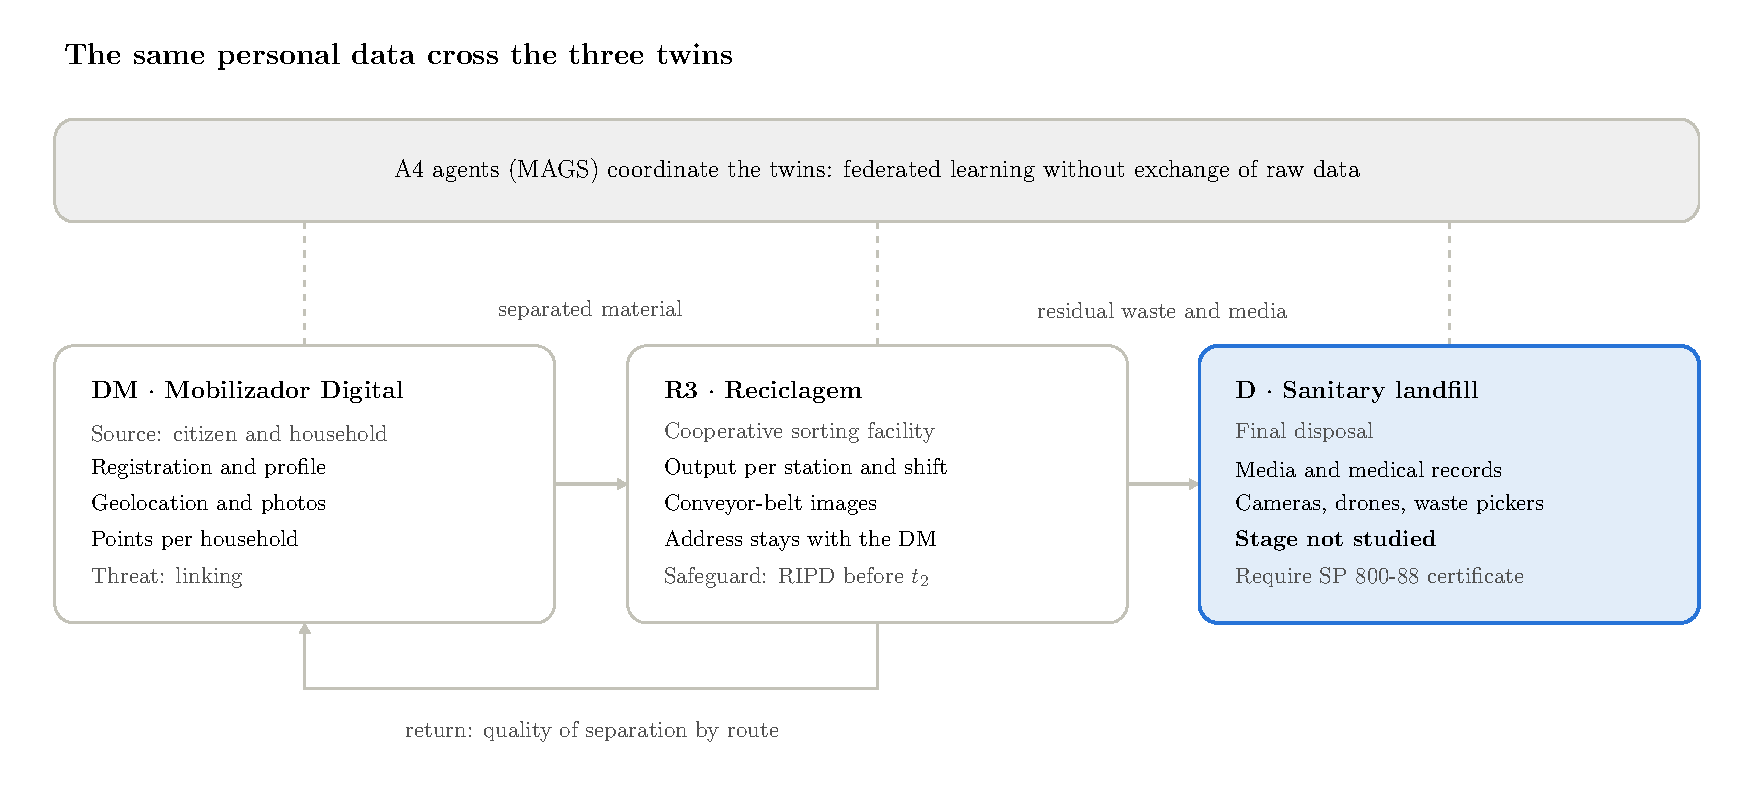
\includegraphics[width=\linewidth]{out/Figura_1_Percurso_Dado_Pessoal_EN.pdf}
\fontetab{Prepared by the author (2026), based on the three base projects.}
\end{figure}

Figure~\ref{fig:percurso} summarizes the path: the data enter the DM, follow the material to R3, return to the DM as quality by route and reach the landfill, the stage that the literature does not study.

Two crossing points deserve attention. The first is the return of quality by route from R3 to the DM: the smaller the route, the closer the information is to the household, and the Landfill project recalls that address, time and weight per generator are attributes that re-identify. The second is the A4 agents, which in the DM coordinate the DM, R2, R3 and DS twins and in R3 coordinate cooperatives, the SLU, buyers and other twins. R3 already proposes the appropriate safeguard---federated learning without exchange of raw data and agreements among cooperatives---but it must hold for the entire network, not only for the Recycling side.

\subsection{Consolidated matrix}

Table~\ref{tab:matriz} brings together, in a single view, the treatment of privacy in each FSPC $\times$ segment cell.

\begin{table}[!htbp]
\centering
\caption{FSPC $\times$ segment cell}
\label{tab:matriz}
\small
\begin{tabularx}{\linewidth}{>{\raggedright\arraybackslash}p{2.2cm} Y Y Y}
\hline
\textbf{Dimension} & \textbf{DM \textperiodcentered{} Mobilizer} & \textbf{R3 \textperiodcentered{} Recycling} & \textbf{D \textperiodcentered{} Landfill}\\
\hline
Function & Profile and scoring by household, implicit & Individual monitoring redesigned into metrics per station & Verified elimination as a function; sanitization certificate\\
Structure & TW named; \textit{blockchain} as an immutable record & Safeguard per agent (A1 to A4) & Sensor density simulated against re-identification\\
Process & Profiling in the first stage; high risk with no treatment stage & RIPD before \dsq{2}; images processed locally & LINDDUN threats by stage; living risk register\\
Context & LGPD declared & Inventory with legal bases; principles in design decisions & Compliance dashboard; LGPD absent from the literature\\
\hline
\end{tabularx}
\fontetab{Prepared by the author (2026).}
\end{table}

Read by columns, the matrix shows a maturity gradient: the DM recognizes the risk, R3 converts it into design decisions and the Landfill converts it into function and indicators. Read by rows, it shows that each segment is strongest in a different dimension, and that the complete description appears only when the three are read together.

\subsection{Edges and faces: where privacy concentrates}

The tetrahedron method allows an additional reading. In R3, the edges and faces that contain Context are the least studied in the literature: FC has 176 records, SC 270 and face FSC only 36. They are also those that concentrate privacy. On edge SC, the LGPD limits the data structure and establishes that the data belong to the cooperative. On face FSC, called institutional architecture by the group, are data governance by the cooperative, roles, consents and data agreements with the SLU and buyers, supported by the MG and TW capabilities.

The Landfill arrives at the same place by another path. The gap that it measures is the privacy Function, but what is missing is precisely the link between Function and Context: the law says that the data must be eliminated, but the literature does not say how to verify that a discarded medium has become unreadable. The convergence suggests that, in the SRS twins, privacy is a property of the relationships with Context, and not of an isolated dimension, and that these relationships are the least covered by the literature.

\subsection{Implications for project management}

The three projects link the twin to project management in different ways. The DM aligns the project with the PMBOK guide through scope, stakeholders, agile life cycle, quality and IT risks---with data security plans---and value delivery, measured by the increase in selective collection and the reduction of logistics costs. R3 distributes effort across the hierarchy of portfolios, programs, projects and operations: the daily schedule and the allocation on the conveyor belt are operations; the implementation of each configuration is a project; the network and the contracts are the P3RD program; and investment priority is the AEDR portfolio. The Landfill proposes that the system twin feed the risk register of the project twin.

For privacy, the Landfill identifies four of the seven PMBOK 8 performance domains that need to be involved, each linked to a function of the NIST Privacy Framework:

\begin{table}[!htbp]
\centering
\caption{NIST Privacy Framework}
\label{tab:nist}
\small
\begin{tabularx}{\linewidth}{>{\raggedright\arraybackslash}p{3.2cm} >{\raggedright\arraybackslash}p{3cm} Y}
\hline
\textbf{PMBOK 8 domain} & \textbf{NIST function} & \textbf{Role in privacy}\\
\hline
Governance & Govern-P & Defines controller and operator among the municipality, consortium, collection company and landfill, and approves the impact assessment report\\
Stakeholders & Communicate-P & Includes data subjects, waste pickers, the surrounding community and the ANPD\\
Resources & Protect-P and Control-P & Treats sensors, cloud and suppliers as resources that process data, with clauses and controls\\
Risk & Identify-P & Each LINDDUN threat becomes a risk with a trigger measured by the twin and goes through the six risk processes\\
\hline
\end{tabularx}
\fontetab{Prepared by the author (2026).}
\end{table}

The same project proposes four criteria for treating Privacy as a domain of its own---its own object of risk (harm to the data subject), its own metrics and units, its own stakeholders and obligations, and activities across the entire life cycle---and a minimum set of indicators, with illustrative targets to be calibrated: 100\% of flows with a legal basis and purpose before operation; zero significant or maximum risks to the data subject without a response; $k \geq 10$ in the data published per generator; a defined and monitored differential privacy budget; 100\% of media batches with verified sanitization; and data subject requests answered within 15 days.

The joint reading shows that these criteria apply to the three segments, and not only to the landfill. The object of risk lies in the DM's households and in R3's waste pickers; the specific metrics apply to the DM's public dashboards and to R3's metrics per station; the specific stakeholders include residents, cooperative members and the ANPD; and the activities across the entire cycle run from profiling in the DM to sanitization at the landfill. R3's RIPD, required before \dsq{2}, is a concrete example of how these criteria become a decision point in the project cycle.

% ------------------------------ 10 LIMITATIONS -------------------------------
\section{LIMITATIONS}

The consolidation inherits the limitations of the three base projects and adds its own.

\textbf{Inherited limitations.} The search protocols differ in database, period and string, and therefore the counts by dimension are not comparable in absolute value. The R3 and DM counts are lexical indicators: they register the presence of the term in the topic, not the quality of the treatment of the dimension, as the Recycling group itself warns. In the Landfill, screening and classification by theme, LINDDUN category and FSPC dimension were performed with regular expressions over title, abstract and keywords, which over-represents themes with broad vocabulary and may miss studies that address privacy without the search terms; the final eligibility decision depends on reading the full text. The DM relies on four articles, one of which (Banik et al., 2025) has a sample of 20 participants. R3 describes the cooperatives generically, with legal bases treated as hypotheses and advancement targets still pending. None of the three twins has been validated in the field.

\textbf{Limitations of the consolidation.} Assigning passages to the cells of the matrix involves judgment, and passages that touch two dimensions were kept where the original project placed them. The privacy points that the projects do not make explicit were derived from the text through the questions of Section 2.1 and are flagged as the consolidation's reading. The paper adds no external sources, which preserves traceability but also means that gaps in the base projects remain gaps here. Finally, the consolidation was carried out with the support of artificial intelligence, under the terms declared in Section 11.

% ------------------------------ 11 AI STATEMENT ------------------------------
\section{STATEMENT ON THE USE OF ARTIFICIAL INTELLIGENCE}

This consolidation was produced with the support of generative artificial intelligence. The research results belong to the groups that produced them; the AI was used to read, organize and draft the synthesis of those results, under human direction and review.

\subsection{Tool and period}

The Claude language model, by Anthropic, was used in a Claude session (Cowork), in October 2026. The session was conducted by a member of the Landfill group, who supplied the three base projects and the PMBOK 8 Guide as files and defined, at each step, the scope and format of the outputs.

\subsection{What the AI did}

\begin{enumerate}
\item \textbf{Reading and extraction.} It extracted the text of the three projects and located the passages that describe function, structure, process and context, with their numerical data and citations.
\item \textbf{Organization.} It assigned the passages to the cells of the FSPC $\times$ segment matrix and compared the cells to identify convergences, divergences and gaps.
\item \textbf{Drafting.} It drafted the text, the tables and the figure of this paper, as well as a preliminary analysis and an A1 poster with the same content.
\item \textbf{Spot check.} In an earlier step, it checked in the PMBOK 8 text the mentions of privacy described by the Landfill project. By decision of the session conductor, the final version is limited to the content of the three base projects.
\end{enumerate}

\subsection{What the AI did not do}

\begin{itemize}
\item It did not run bibliographic searches, did not access the Web of Science or Scopus databases and did not generate new counts, classifications or data. All the numbers cited come from the base projects.
\item It did not add external sources to the base projects. The references cited are those that the groups themselves used.
\item It did not assess whether, or how, each group used AI tools in producing its own project. The authorship, methods and results of each base project are the responsibility of the respective group, which is responsible for declaring the use of AI in its own text.
\item It is not an author of this paper. The AI does not take responsibility for the content and should not be listed as an author.
\end{itemize}

\subsection{Risks and safeguards}

Language models may attribute information to the wrong project, simplify an argument to the point of altering it, or produce plausible statements with no basis in the text. Three safeguards were adopted: (1) the rule of using only the content of the base projects, which makes each statement traceable to one of them; (2) the explicit separation, in Sections 5 to 8, between what the project states and the privacy point derived by the consolidation; and (3) human review before any submission.

Each group is advised to check the cells relating to its segment, especially numbers, citations and legal bases, before the text is presented or submitted. The base projects contain no personal data beyond the names of the authors, and no personal data of third parties were processed in the consolidation.

\subsection{Accountability}

It is up to the authors to review the content generated with the support of AI before submission; after that review, they are fully responsible for it. This statement should be adapted to the policies of the course, the program and the publication venue to which the paper is submitted.

% ------------------------------ 12 CONCLUSIONS -------------------------------
\section{CONCLUSIONS AND FUTURE WORK}

This paper consolidated three projects that describe digital twins of successive segments of the Solid Waste System of the DF, organizing them by the four FSPC dimensions and reading each through the Privacy domain. The answers to the three questions are as follows.

\textbf{Q1. What each segment contributes.} The Mobilizer contributes the origin of the data and the bidirectional loop between citizen and twin; Recycling, the most complete description of the twin in FSPC, the chain of configurations \dsq{k} and privacy safeguards by agent and by data item; the Landfill, the map of threats by stage of the cycle, verified elimination as a function and the link between the system twin and the project twin.

\textbf{Q2. Convergences and divergences.} The three converge on the reference paradigm, on the six DTC capability families, on the bidirectional loop and on the PNRS and LGPD framework. They diverge in the depth with which they treat privacy: the DM recognizes it as a risk, R3 converts it into design decisions and the Landfill converts it into function and indicators. They also diverge in what their searches say about Context: little studied in the recycling and mobilization literature, much studied in the privacy literature, but without reaching rights, institutions and the LGPD.

\textbf{Q3. What only the joint reading reveals.} The same personal data cross the three twins, and their crossing points---the return of quality by route and the A4 network agents---do not belong to any segment in isolation. Privacy concentrates in the relationships with Context (edges FC and SC and face FSC), which are the least studied. And the stage at which the data should cease to exist, final disposal, is the only one without study.

Five lines of work follow from these conclusions, all pointed out or suggested by the base projects:

\begin{enumerate}
\item \textbf{Single register of processing activities.} Unify R3's data inventory with the DM and Landfill flows in one register per twin, with the legal bases validated by the data protection officer, as R3 foresees for the next phase.
\item \textbf{Data agreements among twins.} Extend R3's A4 safeguard---federated learning without exchange of raw data---to the entire network of SRS twins, and define the minimum granularity of the return of quality by route.
\item \textbf{Sanitization protocol.} Develop, as the Landfill proposes, a sanitization verification protocol (NIST SP 800-88) with a certificate traceable to the landfill.
\item \textbf{Dynamic privacy FMEA.} Turn the one-off risk assessment into a living register, updated with operational data from the three twins.
\item \textbf{Field validation.} Validate the descriptions with at least one cooperative and with the SLU, as R3 foresees, and carry out the proof of concept of a project twin at a pilot landfill, as the Landfill foresees.
\end{enumerate}

Read separately, the three projects describe three twins. Read together, they describe a chain, and privacy can be guaranteed only if it is managed as a property of that chain.

% ------------------------------ REFERENCES -----------------------------------
\begin{center}
\textbf{REFERENCES}
\end{center}

\begingroup
\SingleSpacing
\setlength{\parindent}{0pt}
\setlength{\parskip}{12pt}
\raggedright

ALCARAZ, C.; LOPEZ, J. Digital twin: a comprehensive survey of security threats. \textbf{IEEE Communications Surveys \& Tutorials}, v. 24, n. 3, 2022.

BANIK, Bijoy et al. A Mobile Platform for Smart Recycling and Eco-Friendly Sustainable Environment. \textbf{Journal of Social Innovation and Knowledge}, v. 2, p. 150-175, 2025.

BRASIL. Decreto nº 10.936, de 12 de janeiro de 2022. Regulamenta a Lei nº 12.305/2010. Brasília, DF, 2022.

BRASIL. Decreto nº 11.413, de 13 de fevereiro de 2023. Institui o Certificado de Crédito de Reciclagem de Logística Reversa e outros certificados. Brasília, DF, 2023.

BRASIL. Lei nº 12.305, de 2 de agosto de 2010. Institui a Política Nacional de Resíduos Sólidos. Brasília, DF, 2010.

BRASIL. Lei nº 13.709, de 14 de agosto de 2018. Lei Geral de Proteção de Dados Pessoais (LGPD). Brasília, DF, 2018.

BRIGHENTE, A.; CONTI, M.; DI RENZONE, G.; PERUZZI, G.; POZZEBON, A. Security and privacy of smart waste management systems: a cyber-physical system perspective. \textbf{IEEE Internet of Things Journal}, 2024. DOI: 10.1109/JIOT.2023.3322532.

BROOKS, S.; GARCIA, M.; LEFKOVITZ, N.; LIGHTMAN, S.; NADEAU, E. \textbf{An introduction to privacy engineering and risk management in federal systems}. NISTIR 8062. Gaithersburg: NIST, 2017.

CHEN, H.; TUREL, O.; YUAN, Y. E-waste information security protection motivation: the role of optimism bias. \textbf{Information Technology \& People}, 2022. DOI: 10.1108/ITP-09-2019-0458.

DENG, M.; WUYTS, K.; SCANDARIATO, R.; PRENEEL, B.; JOOSEN, W. A privacy threat analysis framework: supporting the elicitation and fulfillment of privacy requirements. \textbf{Requirements Engineering}, v. 16, n. 1, p. 3--32, 2011.

DIGITAL TWIN CONSORTIUM. \textbf{Digital Twin Capabilities Periodic Table (v. 1.2) and AI Agent Capabilities Periodic Table (v. 1.0)}. Boston: DTC, 2025.

FONSECA-MEDRANO, M. C. et al. Characterization of solid wastes as a tool to implement waste management strategies in a university campus. \textbf{International Journal of Sustainability in Higher Education}, v. 21, n. 7, 2020.

FUKAMI, A.; REGAZZONI, F.; GERADTS, Z. Data sanitization on eMMCs. In: \textbf{ASIA AND SOUTH PACIFIC DESIGN AUTOMATION CONFERENCE (ASP-DAC)}, 2023. DOI: 10.1145/3566097.3568349.

GARFINKEL, S. L.; SHELAT, A. Remembrance of data passed: a study of disk sanitization practices. \textbf{IEEE Security \& Privacy}, v. 1, n. 1, p. 17--27, 2003.

GHARAJEDAGHI, J. \textbf{Systems thinking: managing chaos and complexity}. 3. ed. Burlington: Morgan Kaufmann, 2011.

GIEL, R.; DĄBROWSKA, A. Digital twin concept for manual waste sorting management. \textbf{Environment Protection Engineering}, v. 51, n. 1, p. 65--74, 2025. DOI: 10.37190/epe250104.

GRIEVES, M.; VICKERS, J. Digital twin: mitigating unpredictable, undesirable emergent behavior in complex systems. In: KAHLEN, F.-J.; FLUMERFELT, S.; ALVES, A. (ed.). \textbf{Transdisciplinary perspectives on complex systems}. Cham: Springer, 2017.

JOSHI, S.; SHARMA, M.; BARVE, A. Implementation challenges of blockchain technology in closed-loop supply chain: a WEEE management perspective in developing countries. \textbf{Supply Chain Forum: An International Journal}, 2023. DOI: 10.1080/16258312.2022.2135972.

KRITZINGER, W.; KARNER, M.; TRAAR, G.; HENJES, J.; SIHN, W. Digital twin in manufacturing: a categorical literature review and classification. \textbf{IFAC-PapersOnLine}, v. 51, n. 11, p. 1016--1022, 2018. DOI: 10.1016/j.ifacol.2018.08.474.

LEAL, A. E. F. et al. Applications of digital technologies for overcoming challenges in municipal solid waste reverse logistics: a systematic literature review. \textbf{Engenharia Sanitária e Ambiental}, v. 29, 2024.

LI, X. Personal information security risk assessment for e-waste recycling based on Fuzzy-GRA-TOPSIS and FMEA. \textbf{IEEE Transactions on Engineering Management}, 2024. DOI: 10.1109/TEM.2024.3395649.

NISSENBAUM, H. Privacy as contextual integrity. \textbf{Washington Law Review}, v. 79, n. 1, p. 119--157, 2004.

NIST. \textbf{NIST Privacy Framework: a tool for improving privacy through enterprise risk management, version 1.0}. Gaithersburg: NIST, 2020.

NIST. \textbf{SP 800-88 Rev. 1: guidelines for media sanitization}. Gaithersburg: NIST, 2014.

NOLASCO, Elaine et al. Characterization of solid wastes as a tool to implement waste management strategies in a university campus. \textbf{International Journal of Sustainability in Higher Education}, v. 22, n. 4, p. 805-824, 2021.

OLAWADE, D. B. et al. Smart waste management: a paradigm shift enabled by artificial intelligence. \textbf{Waste Management Bulletin}, 2024. DOI: 10.1016/j.wmb.2024.05.001.

OLIVEIRA, G. P.; REIS, M. V. O.; ARCANJO, S. A.; SILVA, W. A. \textbf{Projeto prático: componente de sistema de resíduos sólidos urbanos -- Mobilizador Digital 1}. Brasília: UnB/PPCA, Gestão de Projetos de TI, 2026.

PMI -- PROJECT MANAGEMENT INSTITUTE. \textbf{A guide to the project management body of knowledge (PMBOK guide)}. 8. ed. Newtown Square: PMI, 2025.

PRATA, J.; SIMÕES, C. L.; SIMÕES, R. Improvements to municipal solid waste collection systems using real-time monitoring. \textbf{Sustainability}, v. 17, n. 4, 1405, 2025.

ROCHA, L.; SILVA, E.; GARCIA, H.; FERREIRA, L. \textbf{Privacidade no descarte de resíduos sólidos: atualização SIPA da revisão sobre aterros sanitários sob a ótica FSPC (v2)}. Brasília: UnB/PPCA, Gestão de Projetos de TI, 2026.

ROCHER, L.; HENDRICKX, J. M.; DE MONTJOYE, Y.-A. Estimating the success of re-identifications in incomplete datasets using generative models. \textbf{Nature Communications}, v. 10, art. 3069, 2019.

SOUSA, F. A.; CORREIA, E. B. G.; SILVA, R. I. D.; PAPA, C. E. S. \textbf{Gestão do gêmeo digital de reciclagem em cooperativas sob a ótica da privacidade (SIPA)}. Entrega P2A. Brasília: UnB/PPCA, Gestão de Projetos de TI, 2026.

TAO, F. et al. Digital twin in industry. \textbf{IEEE Transactions on Industrial Informatics}, v. 15, n. 4, p. 2405--2415, 2018.

WANG, H.; ZHENG, L.; XUE, Q.; LI, X. Research on medical waste supervision model and implementation method based on blockchain. \textbf{Security and Communication Networks}, 2022. DOI: 10.1155/2022/5630960.

\endgroup

\end{document}
